\begin{figure}[h]
\centering
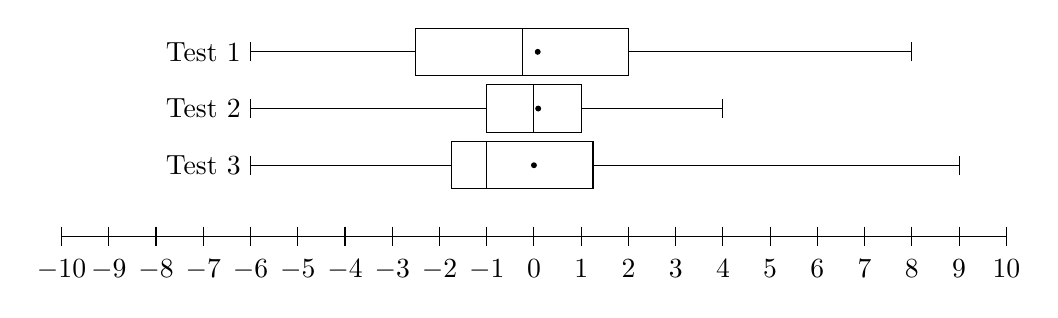
\begin{tikzpicture}[scale=0.6]
%Test 1
\draw (-2.5,3.4) rectangle (2,4.4); % Boks
\draw (-0.25,3.4) -- (-0.25,4.4); % Median streg
\draw (2,3.9) -- (8,3.9); % Fra øvre kvartil til maks
\draw (-2.5,3.9) -- (-6,3.9);% Fra nedre kvartil til min
\draw (8,3.7) -- (8,4.1); % Maksimum vertikal streg
\draw (-6,3.7) -- (-6,4.1); % Minimum vertikal streg
\node[left] at (-6,3.9) {Test 1};
\filldraw[color=black] (0.08,3.9) circle (0.05cm); % Gennemsnittet

%Test 2
\draw (-1,2.2) rectangle (1,3.2); % Boks
\draw (0,2.2) -- (0,3.2); % Median streg
\draw (1,2.7) -- (4,2.7); % Fra øvre kvartil til maks
\draw (-1,2.7) -- (-6,2.7);% Fra nedre kvartil til min
\draw (4,2.5) -- (4,2.9); % Maksimum vertikal streg
\draw (-6,2.5) -- (-6,2.9); % Minimum vertikal streg
\node[left] at (-6,2.7) {Test 2};
\filldraw[color=black] (0.09,2.7) circle (0.05cm); % Gennemsnittet

%Test 3
\draw (-1.75,1) rectangle (1.25,2); % Boks
\draw (-1,1) -- (-1,2); % Median streg
\draw (1.25,1.5) -- (9,1.5); % Fra øvre kvartil til maks
\draw (-1.75,1.5) -- (-6,1.5);% Fra nedre kvartil til min
\draw (9,1.3) -- (9,1.7); % Maksimum vertikal streg
\draw (-6,1.3) -- (-6,1.7); % Minimum vertikal streg
\node[left] at (-6,1.5) {Test 3};
\filldraw[color=black] (0.00,1.5) circle (0.05cm); % Gennemsnittet

% Linje med værdier
\draw (-10,0) -- (10,0);

% Tal på linje
\foreach \x in {-10,-9,...,10} {
	\draw (\x, 0.2) -- (\x, -0.2);
     \node[below] at (\x, -0.3) {$\x$};
}

\end{tikzpicture}
\caption{Boksplot for test af kompas}
\label{kompas:boksplot}
\end{figure}